
%\begin{frame}[t]{Tvarovanie žiadaných hodnôt}
%  \begin{itemize}
%  \item<1-> Dron je stabilizovaný, pilot/ROS náhle chce $r_{\Phi}=$+30$^\circ$ klonenie. Čo sa stane s riadením?
%  \item<2->  Žiadaná hodnota je skokový signál. Derivácia skoku je... D zložka a tým aj vstup do akčných členov vystrelí!
%  \item<3->  Potrebujeme tvarovať vstupy do regulácie \angl{input shaping}, t.j. tvarovať žiadané hodnoty:
%        \begin{itemize}
%  \item Pomalšie vzorkovanie na rýchlejšie (interpolácia) \footnote{ArduCopter 50 Hz $\rightarrow$ 400 Hz \citep{AP:PID}}
%  \item Vyhladenie filtráciou, saturácie
%  \item<4-> Ak hovoríme o manuálnom pilotovaní, tvarovanie určuje aký ``pocit'' je riadiť stroj
%  \end{itemize}
%  \end{itemize}
%
%        \begin{onlyenv}<2>
%  \begin{figure}
%\centering
%  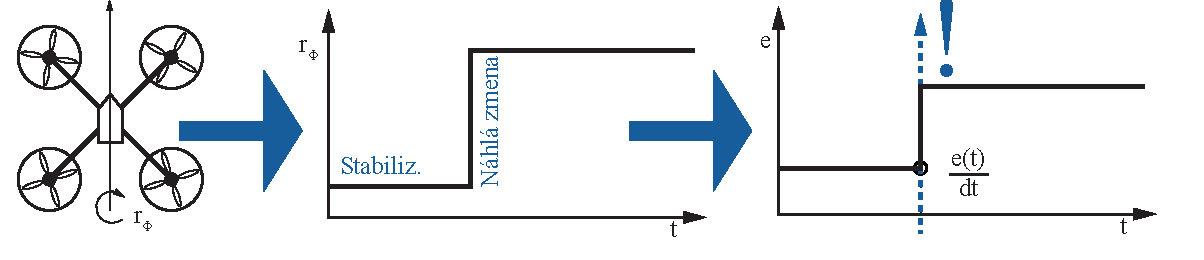
\includegraphics[width=\textwidth]{InputShaping_1}\\
%\end{figure}
%\end{onlyenv}
%
%
%        \begin{onlyenv}<3->
%  \begin{figure}
%\centering
%  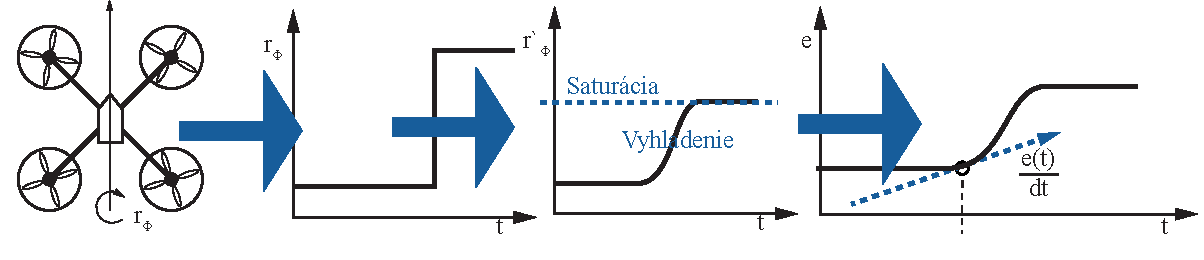
\includegraphics[width=\textwidth]{InputShaping_2}\\
%\end{figure}
%\end{onlyenv}
%
%\end{frame}
%
%\begin{frame}[t]{Inicializácia riadenia}
%\begin{itemize}
%  \item<1-> Ako naštartujeme riadenie? Aká je odchýlka $e(0)$ pri štarte?
%  \item<2-> Kritické pri zmene letových módov \citep{AP:PID,Bresciani2020}
%  \item<3-> Pre ArduCopter \cite{AP:PID}
%    \begin{itemize}
%    \item Nadradené riadenie poloha vs. rýchlosť (P) --- tak aby vstup bol konštantný
%    \item Rýchlosť (PID) --- $e(0)=0$, I zložka s konštantným vstupom, zrátať D pri nastavení žiadanej hodnoty
%\end{itemize}
%
%\end{itemize}
%\end{frame}